%contient des exemples d'homographies traité par nous et ripmap

\sse{Comparaison du Ripmap et de la décomposition géométrique}

Se reporter aux %cite les figure

On peut remarquer que la décomposition permet pour certaines homographies de limiter l'\emph{aliasing} (Homographies 1 et 4). Dans le cas d'une déformation en diagonale elle limite le flou (Homographie 2). Il existe néanmoins des cas où les deux méthodes ont des performances comparables (Homographie 3).

\begin{figure}
\caption{Homographie 1}
\label{Homo1}
\subfigure[Décomposition géométrique]{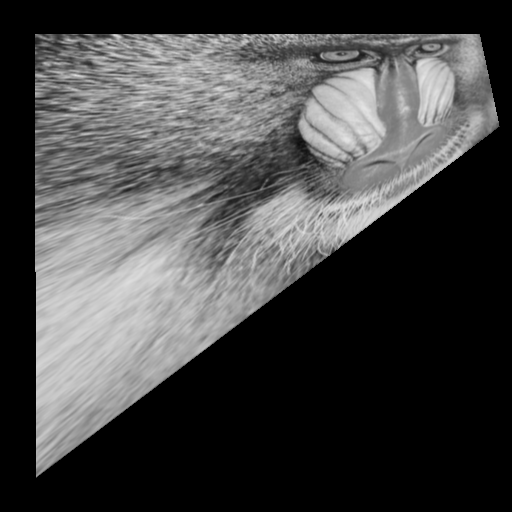
\includegraphics[scale=0.4]{img_f_1.png}}
\subfigure[Ripmap]{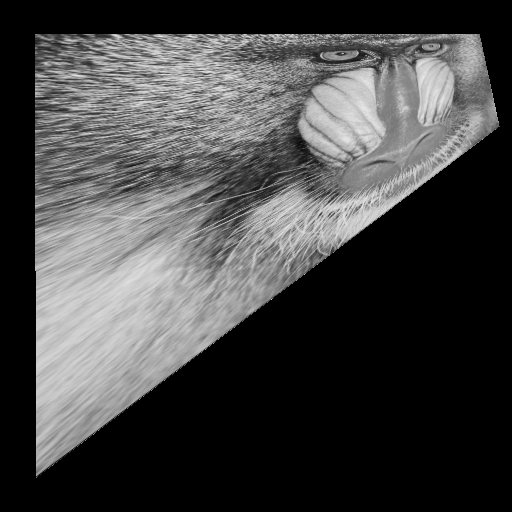
\includegraphics[scale=0.4]{img_ripmap_1.png}}
\end{figure}

\begin{figure}
\caption{Homographie 2}
\label{Homo2}
\subfigure[Décomposition géométrique]{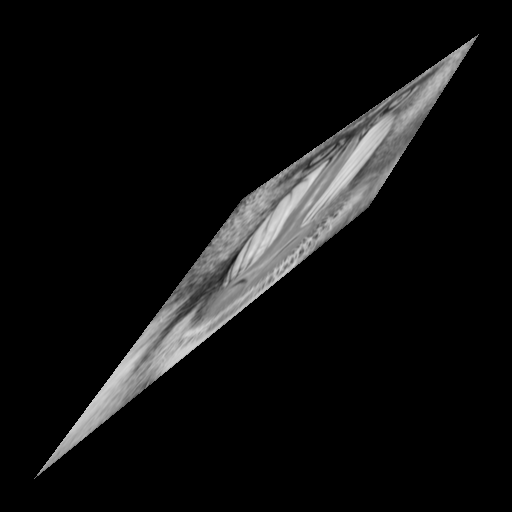
\includegraphics[scale=0.4]{img_f_2.png}}
\subfigure[Ripmap]{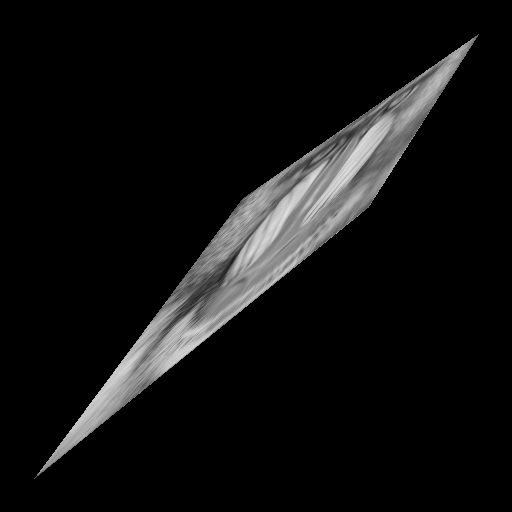
\includegraphics[scale=0.4]{img_ripmap_2.png}}
\end{figure}

\begin{figure}
\caption{Homographie 3}
\label{Homo3}
\subfigure[Décomposition géométrique]{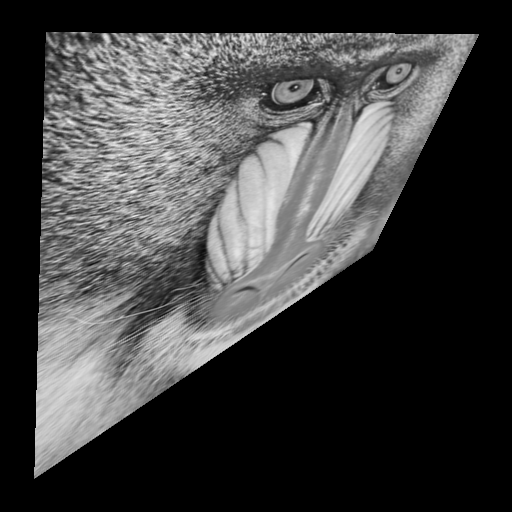
\includegraphics[scale=0.4]{img_f_3.png}}
\subfigure[Ripmap]{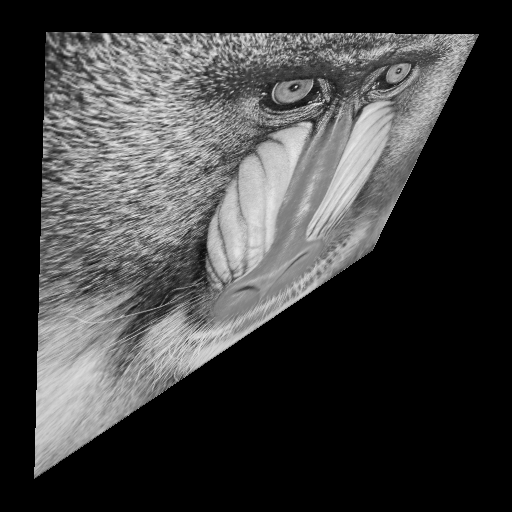
\includegraphics[scale=0.4]{img_ripmap_3.png}}
\end{figure}

\begin{figure}
\caption{Homographie 4}
\label{Homo4}
\subfigure[Décomposition géométrique]{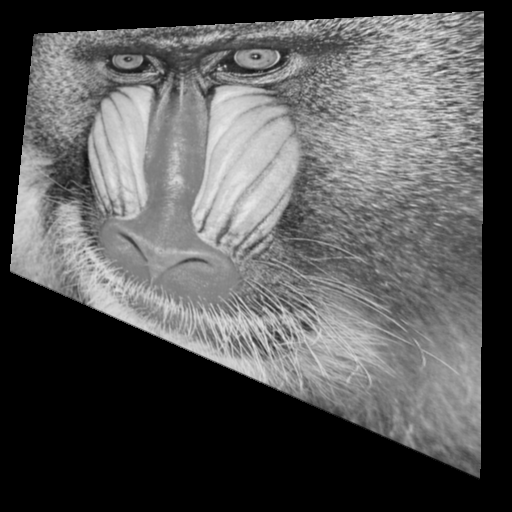
\includegraphics[scale=0.4]{img_f_4.png}}
\subfigure[Ripmap]{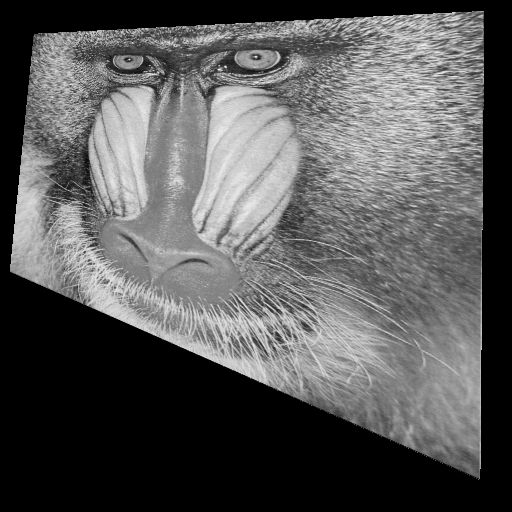
\includegraphics[scale=0.4]{img_ripmap_4.png}}
\end{figure}